\documentclass{beamer}
\usepackage{multicol}
\usepackage{amsmath}
\usepackage[utf8]{inputenc}
%% \setlength{\parindent}{0pt}
%% \setlength{\parskip}{6pt plus 2pt minus 1pt}
%% \setcounter{secnumdepth}{0}

\title{SAT Encodings for the Car Sequencing Problem}
\author{\underline{Valentin Mayer-Eichberger} and Toby Walsh}
\date{08/07/2013 at Pragmatics of SAT}

\usepackage{tikz}
\usetikzlibrary{arrows,shapes}
\usepackage{graphics}
\usepackage[showboxes]{textpos}

\newcommand{\TODO}[1]{\textcolor[rgb]{1.00,0.00,0.00}{#1} }

\newcommand<>{\fullsizegraphic}[1]{
  \begin{textblock*}{0cm}(-1cm,-3.78cm)
  \includegraphics[width=\paperwidth]{#1}
  \end{textblock*}
}

% remove navigation bar
\setbeamertemplate{navigation symbols}{}

% transparent overlays
%\setbeamercovered{transparent}

\newcommand{\todo}[1]{ {\color{red}{#1} }}

\begin{document}
\begin{frame}[fragile]
  \titlepage

\end{frame}
\begin{frame}[fragile]
\frametitle{Car Sequencing}

\begin{multicols}{2}

\includegraphics[scale=0.23]{cars.jpg}

{\tiny Source Wikipedia }
\newpage

\begin{itemize}
\item Cars require different options (air-conditioning, sun-roof, etc.)
\item Is there a production sequence for cars on the assembly line satisfying the sliding capacity constraints?
\item CSPLib Benchmark Nr. 1
\item CP, IP, local search
\end{itemize}

\end{multicols}

\end{frame}
\begin{frame}[fragile]
\frametitle{Car Sequencing: Example}

\begin{itemize}
\itemsep1pt\parskip0pt\parsep0pt
\item
  $C = \{1,2,3\}$ with demand $d_1=3, d_2=2,d_ 3=2$
\item
  $O = \{a,b\}$ with capacity constraints $1/2$ and $1/5$
\item
  Class 1 no restriction
\item
  Class 2 requires option $a$
\item
  Class 3 requires option $a$ and $b$
\end{itemize}

\vspace{0.5cm}

\begin{center}
\begin{small}
\begin{tabular}{c|cccccccc}
Sequence of cars  & 3 & 1 & 2 & 1 & 2 & 1 & 3 \\
\hline
Option a & 1 & - & 1 & - & 1 & - & 1 \\
Option b & 1 & - & - & - & - & - & 1 \\
\end{tabular}
\end{small} 
\end{center}

\pause

\begin{center}

\todo{Car Sequencing is NP-Complete}
\end{center}

\end{frame}
\begin{frame}[fragile]
\frametitle{PB Model}

\begin{itemize}
\itemsep1pt\parskip0pt\parsep0pt
\item
  Boolean variable $c^k_i$: car $k\in C$ is at position $i$
\item
  Boolean variable $o^l_i$: option $l\in O$ is at position $i$
\item
  Demand constraints: $\forall k \in C$ \[\sum^n_{i=1} c^k_i = d_k\]\\
\item
  Capacity constraints: $\forall l \in O$ with ratio $u_l/q_l$
  \[\bigwedge_{i=0}^{n-q_l}(\sum_{j=1}^{q_l} o^l_{i+j} \leq u_l )\]
\end{itemize}

\end{frame}
\begin{frame}[fragile]
\frametitle{PB Model}

And in all positions $i \in \{1\ldots n\}$ of the sequence it must hold:

\begin{itemize}
    \item Link between classes and options: for each $k\in C$ and 
        \begin{align*}
            \forall l \in O_k :\;\; & c^k_i - o^l_i \leq 0 \\
            \forall l \in O \setminus O_k :\;\; &c^k_i + o^l_i \leq 1\\
        \end{align*}
    \item Exactly one car:  $$\sum_{k\in C} c^k_i = 1$$  
\end{itemize}

\end{frame}
\begin{frame}[fragile]
\frametitle{Modelling in CNF}

\begin{itemize}
\itemsep1pt\parskip0pt\parsep0pt
\item
  The PB model is the mostly used model in CP,IP and local search!
\item
  This model with standard translation to CNF (minisat+,clasp \ldots{})
  has bad performance
\item
  Choose the right cardinality translation
\item
  Uniform treatment of classes and options:
  \[ \sum_{i=1}^n o^l_i = d_l =  \sum_{k\in C_l} d_k\]\\
\item
  Global constraint: Cardinality + Sequence
\end{itemize}

\end{frame}
\begin{frame}[fragile]
\frametitle{Sequential Counter: Variables}

\begin{itemize}
    \item Translation of Boolean Cardinality: $$ \sum_{i\in \{1\ldots n\}} x_{i} = d $$ 
    \item  $x_i$ is true iff the object is at position $i$
    \item  $s_{i,j}$ is true iff in the positions $0,1 \ldots i$ the object exists at least $j$ times 
\end{itemize}

\end{frame}
\begin{frame}[fragile]
\frametitle{Sequential Counter: Example}

\begin{center}
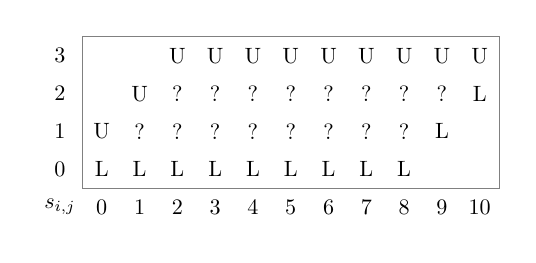
\begin{tikzpicture}[scale=0.8,every node/.style={scale=0.8}]
\node [matrix,ampersand replacement=\&,nodes={minimum size=6mm}]
%,nodes={fill=blue!20,minimum size=5mm}] 
    {
        \node {3}; \& \node (x) { }; \& \node { }; \& \node {U}; \& \node {U}; \& \node {U}; \& \node {U}; \& \node {U}; \& \node {U}; \& \node {U}; \& \node {U}; \& \node {U}; \\
        \node {2}; \& \node { }; \& \node {U}; \& \node {?}; \& \node {?}; \& \node {?}; \& \node {?}; \& \node {?}; \& \node {?}; \& \node {?}; \& \node {?}; \& \node {L}; \\
        \node {1}; \& \node {U}; \& \node {?}; \& \node {?}; \& \node {?}; \& \node {?}; \& \node {?}; \& \node {?}; \& \node {?}; \& \node {?}; \& \node {L}; \& \node { }; \\
        \node {0}; \& \node {L}; \& \node {L}; \& \node {L}; \& \node {L}; \& \node {L}; \& \node {L}; \& \node {L}; \& \node {L}; \& \node {L}; \& \node { }; \& \node (y) { }; \\
        \node {$s_{i,j}$}; \& \node {0}; \& \node {1}; \& \node {2}; \& \node {3}; \& \node {4}; \& \node {5}; \& \node {6}; \& \node {7}; \& \node {8}; \& \node {9}; \& \node {10}; \\
};
\draw[gray] (x.north west) rectangle (y.south east);
\end{tikzpicture}


\end{center}

\vspace{-0.8cm}

Setting $x_2$ and $x_7$ to 1: \vspace{-0.8cm}

\begin{center}
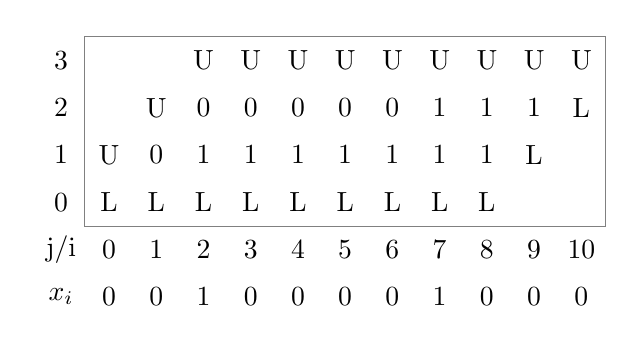
\begin{tikzpicture}
\node [matrix,ampersand replacement=\&,nodes={minimum size=6mm}]
%,nodes={fill=blue!20,minimum size=5mm}] 
    {
        \node {3}; \& \node (x) { }; \& \node { }; \& \node {U}; \& \node {U}; \& \node {U}; \& \node {U}; \& \node {U}; \& \node {U}; \& \node {U}; \& \node {U}; \& \node {U}; \\
        \node {2}; \& \node { }; \& \node {U}; \& \node {0}; \& \node {0}; \& \node {0}; \& \node {0}; \& \node {0}; \& \node {1}; \& \node {1}; \& \node {1}; \& \node {L}; \\
        \node {1}; \& \node {U}; \& \node {0}; \& \node {1}; \& \node {1}; \& \node {1}; \& \node {1}; \& \node {1}; \& \node {1}; \& \node {1}; \& \node {L}; \& \node { }; \\
        \node {0}; \& \node {L}; \& \node {L}; \& \node {L}; \& \node {L}; \& \node {L}; \& \node {L}; \& \node {L}; \& \node {L}; \& \node {L}; \& \node { }; \& \node (y) { }; \\
        \node {j/i}; \& \node {0}; \& \node {1}; \& \node {2}; \& \node {3}; \& \node {4}; \& \node {5}; \& \node {6}; \& \node {7}; \& \node {8}; \& \node {9}; \& \node {10}; \\
        \node {$x_{i}$}; \& \node {0}; \& \node {0}; \& \node {1}; \& \node {0}; \& \node {0}; \& \node {0}; \& \node {0}; \& \node {1}; \& \node {0}; \& \node {0}; \& \node {0}; \\
};
\draw[gray] (x.north west) rectangle (y.south east);
\end{tikzpicture}


\end{center}

\end{frame}
\begin{frame}[fragile]
\frametitle{Sequential Counter}

\begin{center}

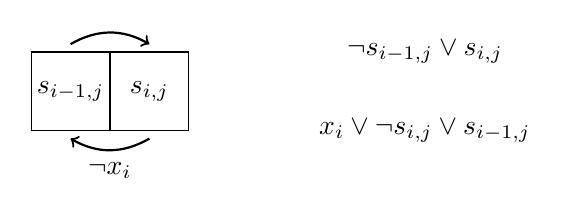
\begin{tikzpicture}[node distance=1cm, auto,]

\coordinate (A) at (0.5,1.1);
\coordinate (B) at (1.5,1.1);
\coordinate (C) at (0.5,-0.1);
\coordinate (D) at (1.5,-0.1);

\draw (0, 0) rectangle (1, 1);
\draw (1, 0) rectangle (2, 1);
\draw[->,thick] (A) to [bend left] (B);
\draw[->,thick] (D) to [bend left] (C);


\node at (0.5,0.5) {$s_{i-1,j}$};
\node at (1.5,0.5) {$s_{i,j}$};
%\node at (1,1.5) {test};
\node at (1,-0.5) {$\neg x_i$};

\node at (5,1) {$\neg s_{i-1,j} \vee s_{i,j}$};
\node at (5,0) {$x_{i} \vee \neg s_{i,j} \vee s_{i-1,j}$};

\end{tikzpicture}

\vspace{1cm}

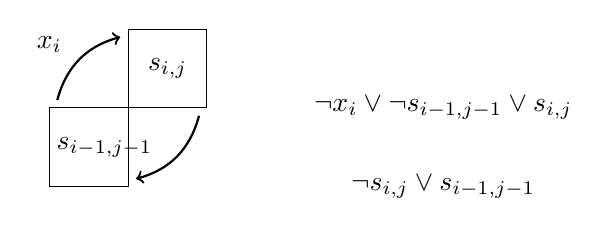
\begin{tikzpicture}[node distance=1cm, auto,]

\coordinate (A) at (0.1,1.1);
\coordinate (B) at (0.9,1.9);
\coordinate (C) at (1.1,0.1);
\coordinate (D) at (1.9,0.9);

\draw (0, 0) rectangle (1, 1);
\draw (1, 1) rectangle (2, 2);
\draw[->,thick] (A) to [bend left] (B);
\draw[->,thick] (D) to [bend left] (C);

\node at (0.7,0.5) {$s_{i-1,j-1}$};
\node at (1.5,1.5) {$s_{i,j}$};
\node at (0,1.8) {$x_i$};
%\node at (2,0) {test};

\node at (5,1) {$\neg x_{i} \vee \neg s_{i-1,j-1} \vee s_{i,j}$};
\node at (5,0) {$\neg s_{i,j} \vee s_{i-1,j-1}$};

\end{tikzpicture}
\end{center}

\begin{itemize}
\itemsep1pt\parskip0pt\parsep0pt
\item
  This idea can translate all cardinality constraints
\end{itemize}

\end{frame}
\begin{frame}[fragile]
\frametitle{Demand Constraint + Capacity Constraint}

\[ (\sum_{i=1}^n x_{i} = d) \wedge \bigwedge_{i=0}^{n-q}(\sum_{l=1}^q x_{i+l} \leq u )\]

\pause
\vspace{1cm}

\begin{center}

\begin{tikzpicture}[node distance=1cm, auto,]

\coordinate (A) at (0.5,1.1);
\coordinate (B) at (3.9,3.5);

\draw (0, 0) rectangle (1, 1);
\draw (4, 3) rectangle (5, 4);
\draw[->,thick] (B) to [bend right] (A);

\draw[dashed] (4.5,0.5) -- (4.5,3);
\draw[dashed] (1.5,0.5) -- (4.5,0.5);

\node at (0.7,0.5) {$s_{i-q,j-u}$};
\node at (4.5,3.5) {$s_{i,j}$};

\node at (4.1,2) {$u$};
\node at (2.5,0) {$q$};

\node at (8,2) {$\neg s_{i,j} \vee s_{i-q,j-u}$};

\end{tikzpicture}

\end{center}

\end{frame}
\begin{frame}[fragile]
\frametitle{Capacity Constraints: Example}

Capacity constraint $4/8$, demand $d=12$ on a sequence of 22 variables:

\begin{tikzpicture}[scale=0.8]
\node [matrix,ampersand replacement=\&,nodes={minimum size=6mm}]
%,nodes={fill=blue!20,minimum size=5mm}] 
    {
\node{13}; \& \node (x) { }; \& \node { }; \& \node { }; \& \node { }; \& \node { }; \& \node { }; \& \node { }; \& \node { }; \& \node { }; \& \node { }; \& \node { }; \& \node { }; \& \node { }; \& \node { }; \& \node { }; \& \node { }; \& \node { }; \& \node { }; \& \node { }; \& \node { }; \& \node {U}; \& \node {U}; \& \node {U}; \\
\node{12}; \& \node { }; \& \node { }; \& \node { }; \& \node { }; \& \node { }; \& \node { }; \& \node { }; \& \node { }; \& \node { }; \& \node { }; \& \node { }; \& \node { }; \& \node { }; \& \node { }; \& \node { }; \& \node { }; \& \node { }; \& \node { }; \& \node { }; \& \node {U}; \& \node {?}; \& \node {?}; \& \node {L}; \\
\node{11}; \& \node { }; \& \node { }; \& \node { }; \& \node { }; \& \node { }; \& \node { }; \& \node { }; \& \node { }; \& \node { }; \& \node { }; \& \node { }; \& \node { }; \& \node { }; \& \node { }; \& \node { }; \& \node { }; \& \node { }; \& \node { }; \& \node {U}; \& \node {?}; \& \node {?}; \& \node {L}; \& \node { }; \\
\node{10}; \& \node { }; \& \node { }; \& \node { }; \& \node { }; \& \node { }; \& \node { }; \& \node { }; \& \node { }; \& \node { }; \& \node { }; \& \node { }; \& \node { }; \& \node { }; \& \node { }; \& \node { }; \& \node { }; \& \node { }; \& \node {U}; \& \node {?}; \& \node {?}; \& \node {L}; \& \node { }; \& \node { }; \\
\node{9}; \& \node { }; \& \node { }; \& \node { }; \& \node { }; \& \node { }; \& \node { }; \& \node { }; \& \node { }; \& \node { }; \& \node { }; \& \node { }; \& \node { }; \& \node {U}; \& \node {U}; \& \node {U}; \& \node {U}; \& \node {U}; \& \node {?}; \& \node {?}; \& \node {L}; \& \node { }; \& \node { }; \& \node { }; \\
\node{8}; \& \node { }; \& \node { }; \& \node { }; \& \node { }; \& \node { }; \& \node { }; \& \node { }; \& \node { }; \& \node { }; \& \node { }; \& \node { }; \& \node {U}; \& \node {?}; \& \node {?}; \& \node {L}; \& \node {L}; \& \node {L}; \& \node {L}; \& \node {L}; \& \node { }; \& \node { }; \& \node { }; \& \node { }; \\
\node{7}; \& \node { }; \& \node { }; \& \node { }; \& \node { }; \& \node { }; \& \node { }; \& \node { }; \& \node { }; \& \node { }; \& \node { }; \& \node {U}; \& \node {?}; \& \node {?}; \& \node {L}; \& \node { }; \& \node { }; \& \node { }; \& \node { }; \& \node { }; \& \node { }; \& \node { }; \& \node { }; \& \node { }; \\
\node{6}; \& \node { }; \& \node { }; \& \node { }; \& \node { }; \& \node { }; \& \node { }; \& \node { }; \& \node { }; \& \node { }; \& \node {U}; \& \node {?}; \& \node {?}; \& \node {L}; \& \node { }; \& \node { }; \& \node { }; \& \node { }; \& \node { }; \& \node { }; \& \node { }; \& \node { }; \& \node { }; \& \node { }; \\
\node{5}; \& \node { }; \& \node { }; \& \node { }; \& \node { }; \& \node {U}; \& \node {U}; \& \node {U}; \& \node {U}; \& \node {U}; \& \node {?}; \& \node {?}; \& \node {L}; \& \node { }; \& \node { }; \& \node { }; \& \node { }; \& \node { }; \& \node { }; \& \node { }; \& \node { }; \& \node { }; \& \node { }; \& \node { }; \\
\node{4}; \& \node { }; \& \node { }; \& \node { }; \& \node {U}; \& \node {?}; \& \node {?}; \& \node {L}; \& \node {L}; \& \node {L}; \& \node {L}; \& \node {L}; \& \node { }; \& \node { }; \& \node { }; \& \node { }; \& \node { }; \& \node { }; \& \node { }; \& \node { }; \& \node { }; \& \node { }; \& \node { }; \& \node { }; \\
\node{3}; \& \node { }; \& \node { }; \& \node {U}; \& \node {?}; \& \node {?}; \& \node {L}; \& \node { }; \& \node { }; \& \node { }; \& \node { }; \& \node { }; \& \node { }; \& \node { }; \& \node { }; \& \node { }; \& \node { }; \& \node { }; \& \node { }; \& \node { }; \& \node { }; \& \node { }; \& \node { }; \& \node { }; \\
\node{2}; \& \node { }; \& \node {U}; \& \node {?}; \& \node {?}; \& \node {L}; \& \node { }; \& \node { }; \& \node { }; \& \node { }; \& \node { }; \& \node { }; \& \node { }; \& \node { }; \& \node { }; \& \node { }; \& \node { }; \& \node { }; \& \node { }; \& \node { }; \& \node { }; \& \node { }; \& \node { }; \& \node { }; \\
\node{1}; \& \node {U}; \& \node {?}; \& \node {?}; \& \node {L}; \& \node { }; \& \node { }; \& \node { }; \& \node { }; \& \node { }; \& \node { }; \& \node { }; \& \node { }; \& \node { }; \& \node { }; \& \node { }; \& \node { }; \& \node { }; \& \node { }; \& \node { }; \& \node { }; \& \node { }; \& \node { }; \& \node { }; \\
\node{0}; \& \node {L}; \& \node {L}; \& \node {L}; \& \node { }; \& \node { }; \& \node { }; \& \node { }; \& \node { }; \& \node { }; \& \node { }; \& \node { }; \& \node { }; \& \node { }; \& \node { }; \& \node { }; \& \node { }; \& \node { }; \& \node { }; \& \node { }; \& \node { }; \& \node { }; \& \node { }; \& \node (y) { }; \\
\node{j/i}; \& \node {0}; \& \node {1}; \& \node {2}; \& \node {3}; \& \node {4}; \& \node {5}; \& \node {6}; \& \node {7}; \& \node {8}; \& \node {9}; \& \node {10}; \& \node {11}; \& \node {12}; \& \node {13}; \& \node {14}; \& \node {15}; \& \node {16}; \& \node {17}; \& \node {18}; \& \node {19}; \& \node {20}; \& \node {21}; \& \node {22}; \\
\node{$x_i$}; \& \node { }; \& \node { }; \& \node { }; \& \node { }; \&
        \node { }; \& \node { }; \& \node { }; \& \node {\textbf{0}}; \&
        \node {\textbf{0}}; \& \node { }; \& \node { }; \& \node { }; \&
        \node { }; \& \node { }; \& \node { }; \& \node {\textbf{0}}; \&
        \node {\textbf{0}}; \& \node { }; \& \node { }; \& \node { }; \& \node { }; \& \node { }; \& \node { }; \\
};
\draw[gray] (x.north west) rectangle (y.south east);
\end{tikzpicture}



\end{frame}
\begin{frame}[fragile]
\frametitle{Capacity Constraints: Example}

Partial Assignment: $x_{1}$ and $x_{13}$ to true and $x_{12}$, $x_{14}$
and $x_{21}$ to false.

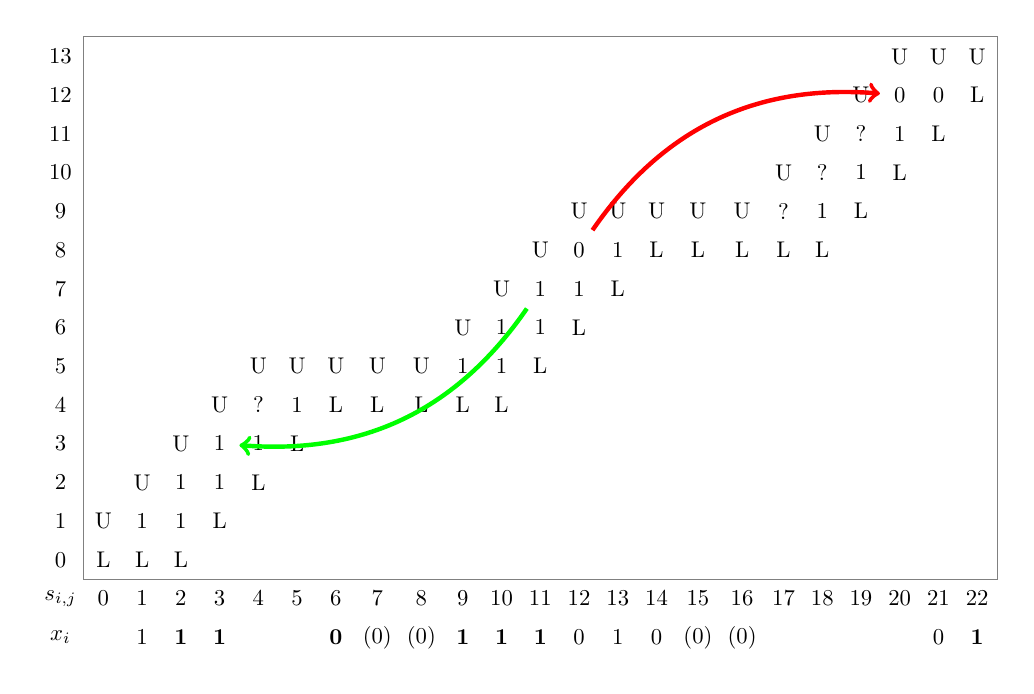
\begin{tikzpicture}[scale=0.82,every node/.style={scale=0.82}]
\node [matrix,ampersand replacement=\&,nodes={minimum size=6mm}]
    {
\node {13}; \& \node (x) { }; \& \node { }; \& \node { }; \& \node { }; \& \node { }; \& \node { }; \& \node { }; \& \node { }; \& \node { }; \& \node { }; \& \node { }; \& \node { }; \& \node { }; \& \node { }; \& \node { }; \& \node { }; \& \node { }; \& \node { }; \& \node { }; \& \node { }; \& \node {U}; \& \node {U}; \& \node {U}; \\
\node {12}; \& \node { }; \& \node { }; \& \node { }; \& \node { }; \&
        \node { }; \& \node { }; \& \node { }; \& \node { }; \& \node {
    }; \& \node { }; \& \node { }; \& \node { }; \& \node { }; \& \node
        { }; \& \node { }; \& \node { }; \& \node { }; \& \node { }; \&
        \node { }; \& \node {U}; \& \node (b) {0}; \& \node {0}; \& \node {L}; \\
\node {11}; \& \node { }; \& \node { }; \& \node { }; \& \node { }; \& \node { }; \& \node { }; \& \node { }; \& \node { }; \& \node { }; \& \node { }; \& \node { }; \& \node { }; \& \node { }; \& \node { }; \& \node { }; \& \node { }; \& \node { }; \& \node { }; \& \node {U}; \& \node {?}; \& \node {1}; \& \node {L}; \& \node { }; \\
\node {10}; \& \node { }; \& \node { }; \& \node { }; \& \node { }; \& \node { }; \& \node { }; \& \node { }; \& \node { }; \& \node { }; \& \node { }; \& \node { }; \& \node { }; \& \node { }; \& \node { }; \& \node { }; \& \node { }; \& \node { }; \& \node {U}; \& \node {?}; \& \node {1}; \& \node {L}; \& \node { }; \& \node { }; \\
\node {9}; \& \node { }; \& \node { }; \& \node { }; \& \node { }; \& \node { }; \& \node { }; \& \node { }; \& \node { }; \& \node { }; \& \node { }; \& \node { }; \& \node { }; \& \node {U}; \& \node {U}; \& \node {U}; \& \node {U}; \& \node {U}; \& \node {?}; \& \node {1}; \& \node {L}; \& \node { }; \& \node { }; \& \node { }; \\
\node {8}; \& \node { }; \& \node { }; \& \node { }; \& \node { }; \& \node { }; \& \node { }; \& \node { }; \& \node { }; \& \node { }; \& \node { }; \& \node { }; \& \node {U}; \& \node (a) {0}; \& \node {1}; \& \node {L}; \& \node {L}; \& \node {L}; \& \node {L}; \& \node {L}; \& \node { }; \& \node { }; \& \node { }; \& \node { }; \\
\node {7}; \& \node { }; \& \node { }; \& \node { }; \& \node { }; \&
        \node { }; \& \node { }; \& \node { }; \& \node { }; \& \node {
    }; \& \node { }; \& \node {U}; \& \node (c) {1}; \& \node {1}; \& \node {L}; \& \node { }; \& \node { }; \& \node { }; \& \node { }; \& \node { }; \& \node { }; \& \node { }; \& \node { }; \& \node { }; \\
\node {6}; \& \node { }; \& \node { }; \& \node { }; \& \node { }; \& \node { }; \& \node { }; \& \node { }; \& \node { }; \& \node { }; \& \node {U}; \& \node {1}; \& \node {1}; \& \node {L}; \& \node { }; \& \node { }; \& \node { }; \& \node { }; \& \node { }; \& \node { }; \& \node { }; \& \node { }; \& \node { }; \& \node { }; \\
\node {5}; \& \node { }; \& \node { }; \& \node { }; \& \node { }; \& \node {U}; \& \node {U}; \& \node {U}; \& \node {U}; \& \node {U}; \& \node {1}; \& \node {1}; \& \node {L}; \& \node { }; \& \node { }; \& \node { }; \& \node { }; \& \node { }; \& \node { }; \& \node { }; \& \node { }; \& \node { }; \& \node { }; \& \node { }; \\
\node {4}; \& \node { }; \& \node { }; \& \node { }; \& \node {U}; \& \node {?}; \& \node {1}; \& \node {L}; \& \node {L}; \& \node {L}; \& \node {L}; \& \node {L}; \& \node { }; \& \node { }; \& \node { }; \& \node { }; \& \node { }; \& \node { }; \& \node { }; \& \node { }; \& \node { }; \& \node { }; \& \node { }; \& \node { }; \\
        \node {3}; \& \node { }; \& \node { }; \& \node {U}; \& \node
        (d) {1}; \& \node {1}; \& \node {L}; \& \node { }; \& \node { }; \& \node { }; \& \node { }; \& \node { }; \& \node { }; \& \node { }; \& \node { }; \& \node { }; \& \node { }; \& \node { }; \& \node { }; \& \node { }; \& \node { }; \& \node { }; \& \node { }; \& \node { }; \\
\node {2}; \& \node { }; \& \node {U}; \& \node {1}; \& \node {1}; \& \node {L}; \& \node { }; \& \node { }; \& \node { }; \& \node { }; \& \node { }; \& \node { }; \& \node { }; \& \node { }; \& \node { }; \& \node { }; \& \node { }; \& \node { }; \& \node { }; \& \node { }; \& \node { }; \& \node { }; \& \node { }; \& \node { }; \\
\node {1}; \& \node {U}; \& \node {1}; \& \node {1}; \& \node {L}; \& \node { }; \& \node { }; \& \node { }; \& \node { }; \& \node { }; \& \node { }; \& \node { }; \& \node { }; \& \node { }; \& \node { }; \& \node { }; \& \node { }; \& \node { }; \& \node { }; \& \node { }; \& \node { }; \& \node { }; \& \node { }; \& \node { }; \\
\node {0}; \& \node {L}; \& \node {L}; \& \node {L}; \& \node { }; \& \node { }; \& \node { }; \& \node { }; \& \node { }; \& \node { }; \& \node { }; \& \node { }; \& \node { }; \& \node { }; \& \node { }; \& \node { }; \& \node { }; \& \node { }; \& \node { }; \& \node { }; \& \node { }; \& \node { }; \& \node { }; \& \node (y) { }; \\
\node {$s_{i,j}$}; \& \node {0}; \& \node {1}; \& \node {2}; \& \node {3}; \& \node {4}; \& \node {5}; \& \node {6}; \& \node {7}; \& \node {8}; \& \node {9}; \& \node {10}; \& \node {11}; \& \node {12}; \& \node {13}; \& \node {14}; \& \node {15}; \& \node {16}; \& \node {17}; \& \node {18}; \& \node {19}; \& \node {20}; \& \node {21}; \& \node {22}; \\
        \node{$x_i$}; \& \node {}; \& \node {1}; \& \node {\textbf{1}}; \& \node { \textbf{1}}; \& \node { }; \& \node { }; \& \node {\textbf{0} }; \& \node {(0)}; \& \node {(0)}; \& \node {\textbf{1} }; \& \node {\textbf{1} }; \& \node {\textbf{1} }; \& \node {0}; \& \node {1}; \& \node {0}; \& \node {(0)}; \& \node {(0)}; \& \node { }; \& \node { }; \& \node { }; \& \node { }; \& \node {0}; \& \node {\textbf{1}}; \\
};
\draw[red,ultra thick,->] (a) to [bend left] (b); 
\draw[green, ultra thick,->] (c) to [bend left] (d); 
\draw[gray] (x.north west) rectangle (y.south east);
\end{tikzpicture}       


\end{frame}
\begin{frame}[fragile]
\frametitle{Discussion: Related Work}

\begin{itemize}
\itemsep1pt\parskip0pt\parsep0pt
\item
  Sinz: Sequential Counter CNF \cite{Sinz05}
\item
  Een and Soerensson: Translation through BDDs to CNF \cite{Een06}
\item
  Bacchus: Decomposition through DFAs to CNF \cite{Bacchus07}
\item
  Brand et al: Decomposition to cumulative sums for CP \cite{Brand07}
\item
  Siala et al: Linear time propagator for CP \cite{Siala12}
\end{itemize}

\end{frame}
\begin{frame}[fragile]
\frametitle{A Trick for Lower Bounds (\cite{Gent98})}

\begin{table}
\tiny
    %%%%%%%%%%%%%%%%%%%%%%%%%%%%%%%%%%%%%%%%%%%%%%%%%%%%%%%%%%%%%%%%%%%%%%
%%                                                                  %%
%%  This is a LaTeX2e table fragment exported from Gnumeric.        %%
%%                                                                  %%
%%%%%%%%%%%%%%%%%%%%%%%%%%%%%%%%%%%%%%%%%%%%%%%%%%%%%%%%%%%%%%%%%%%%%%
\begin{tabular*}{1\linewidth}{@{\extracolsep{\fill}} c|rrrrrrrrrrrr}
class	&0	&1	&2	&3	&4	&5	&6	&7	&8	&9	&10	&11	\\
demand	&9	&4	&22	&2	&1	&62	&31	&4	&24	&4	&3	&36	\\
  \hline                        
0: $1/2$	&-	&-	&-	&-	&-	&-	&-	&-	&-	&-	&-  &x \\
1: $2/3$	&-	&-	&-	&-	&-	&x	&x	&x	&x	&x	&x  &- \\
2: $1/3$	&-	&-	&x	&x	&x	&-	&-	&-	&x	&x	&x  &- \\
3: $2/5$	&-	&x	&-	&-	&x	&-	&x	&x	&-	&-	&x  &- \\
4: $1/5$	&x	&x	&-	&x	&x	&-	&-	&x	&-	&x	&x  &- \\
\end{tabular*}

\vspace{1cm}

\begin{tabular*}{1\linewidth}{@{\extracolsep{\fill}} c|rrrrrrrrrrrrr}
class		&12	&13	&14	&15	&16	&17	&18	&19	&20	&\textbf{21} &22 &\textbf{23}\\
demand		&3	&25	&3	&8	&5	&2	&6	&21	&5	&\textbf{7 } &11 &\textbf{2}\\
  \hline
0: $1/2$	&x	&x	&x	&x	&x	&x	&x	&x	&x	&\textbf{x } &x	 &\textbf{x}\\
1: $2/3$	&-	&-	&-	&-	&-	&-	&x	&x	&x	&\textbf{x } &x	 &\textbf{x}\\
2: $1/3$	&-	&-	&-	&x	&x	&x	&-	&-	&-	&\textbf{x } &x	 &\textbf{x}\\
3: $2/5$	&-	&x	&x	&-	&-	&x	&-	&x	&x	&\textbf{- } &x	 &\textbf{x}\\
4: $1/5$	&x	&-	&x	&-	&x	&x	&x	&-	&x	&\textbf{x } &-	 &\textbf{x}\\
\end{tabular*}

    \label{tab:2}
\end{table}

\begin{itemize}
\itemsep1pt\parskip0pt\parsep0pt
\item
  Class 21 and 23 have option 0,1,2,4 with a total demand of 9
\item
  All other classes share at least one option with 21 and 23
\item
  Potential neighbours of 21 and 23?
\end{itemize}

\end{frame}
\begin{frame}[fragile]
\frametitle{Results on CSPLib}

\begin{center}
\begin{tabular}{ l|ccccc }
	&E1	&E2	&E3	&ASP	&PB\\
\hline
\#solved UNSAT	&{\bf 17}	&15	&{\bf 17} &10	&8\\
\#fastest UNSAT	&{\bf 5}	&4	&4	&0	&4\\
\#solved SAT	&{\bf 11}	&{\bf 11}	&\bf{11}	&7	&2\\
\#fastest SAT	&0	&4	&{\bf 7}	&0	&0\\
\hline
\end{tabular}

\end{center}

\vspace{1cm}

\begin{itemize}
\itemsep1pt\parskip0pt\parsep0pt
\item
  More propagation important for SAT instances, not so much for UNSAT
\item
  Combination of SAT and the Trick shows many lower bounds (additional
  empty cars)
\end{itemize}

\end{frame}
\begin{frame}[fragile]
\frametitle{Conclusions and Future Work}

\begin{itemize}
\itemsep1pt\parskip0pt\parsep0pt
\item
  SAT can be very competitive on CP benchmarks
\item
  SAT is very strong on proving lower bounds
\item
  Global Constraints motivate for encodings
\item
  Choosing the right encoding of cardinality constraints is crucial
\end{itemize}

Future work:

\begin{itemize}
\itemsep1pt\parskip0pt\parsep0pt
\item
  Comparison to CP and IP
\item
  Theoretical analysis of the decompositions and usage in other domains
\item
  Exponential encoding in the number of options?
\end{itemize}

\appendix
\newcounter{finalframe} \setcounter{finalframe}{\value{framenumber}}

\end{frame}
\begin{frame}[fragile]
\frametitle{End}

Thank you very much

\end{frame}
\begin{frame}[fragile]
\frametitle{Bibliography}

\bibliography{p}

\bibliographystyle{plain}

\end{frame}
\begin{frame}[fragile]
\frametitle{Backupslides}

\end{frame}
\begin{frame}[fragile]
\frametitle{Sequential Counter: Comparison to \todo{Sinzs AtMost}}

$\forall i \in \{1\ldots n\}$ $\forall j \in\{0 \ldots d+1\}$: \todo{
\begin{equation} \label{eq:1}
    \neg s_{i-1,j} \vee s_{i,j}
\end{equation}
}

\begin{equation} \label{eq:2}
    x_{i} \vee \neg s_{i,j} \vee s_{i-1,j}
\end{equation}

$\forall {i \in \{1\ldots n\}} \forall {j\in \{1\ldots d+1\}}$:

\begin{equation} \label{eq:3}
    \neg s_{i,j} \vee s_{i-1,j-1}
\end{equation}

\todo{
\begin{equation} \label{eq:4}
    \neg x_{i} \vee \neg s_{i-1,j-1} \vee s_{i,j}
\end{equation}

\begin{equation} \label{eq:5}
     s_{0,0} \wedge \neg s_{0,1} \wedge \neg s_{n,d+1}
\end{equation}
}

\end{frame}
\begin{frame}[fragile]
\frametitle{SAT instances}

%%%%%%%%%%%%%%%%%%%%%%%%%%%%%%%%%%%%%%%%%%%%%%%%%%%%%%%%%%%%%%%%%%%%%%
%%                                                                  %%
%%  This is a LaTeX2e table fragment exported from Gnumeric.        %%
%%                                                                  %%
    %%%%%%%%%%%%%%%%%%%%%%%%%%%%%%%%%%%%%%%%%%%%%%%%%%%%%%%%%%%%%%%%%%%%%%
\begin{tabular}{ lc|ccc }
Instance &Result &E1	    &E2	    &E3 \\
    \hline
4/72	&SAT	&0.2	&0.2	&0.1\\
6/76	&UNSAT	&6.5	&8.2	&18.3\\
10/93	&UNSAT	&8.8	&17.3	&17.5\\
16/81	&SAT	&0.3	&0.1	&0.1\\
19/71	&-	&-	&-	&-\\
21/90	&UNSAT	&157.9	&93.8	&288.3\\
36/92	&UNSAT	&23.5	&54.2	&57.9\\
41/66	&SAT	&0.0	&0.0	&0.1\\
26/82	&SAT	&0.6	&0.1	&0.1\\
 & & & &  \\
200-01	&SAT	&76.5	&68.1	&7.5\\
200-02	&-	&-	&-	&-\\
200-03	&UNSAT	&26.9	&20.5	&35.1\\
200-04	&UNSAT	&116.2	&372.2	&15.5\\
200-05	&UNSAT	&515.5	&-	&1381.4\\
200-06	&-	&-	&-	&-\\
200-07	&SAT	&8.1	&2.2	&0.8\\
200-08	&-	&-	&-	&-\\
200-09	&UNSAT	&192.9	&-	&-\\
200-10	&UNSAT	&2.7	&5.7	&5.1\\
    \hline
\end{tabular}


\end{frame}
\begin{frame}[fragile]
\frametitle{UNSAT instances}

\small

%%%%%%%%%%%%%%%%%%%%%%%%%%%%%%%%%%%%%%%%%%%%%%%%%%%%%%%%%%%%%%%%%%%%%%
%%                                                                  %%
%%  This is a LaTeX2e table fragment exported from Gnumeric.        %%
%%                                                                  %%
%%%%%%%%%%%%%%%%%%%%%%%%%%%%%%%%%%%%%%%%%%%%%%%%%%%%%%%%%%%%%%%%%%%%%%
%\begin{tabular}{ lc|ccc }
%Instance &Result &E1	    &E2	    &E3 \\
%    \hline
%300-01	&SAT	&180.9	&8.0	&38.1\\
%300-02	&-	&-	&-	&-\\
%300-03	&UNSAT	&613.0	&-	&1276.7\\
%300-04	&UNSAT	&4.9	&44.4	&3.7\\
%300-05	&UNSAT	&0.6	&3.3	&0.8\\
%300-06	&-	&-	&-	&-\\
%300-07	&SAT	&173.6	&15.8	&8.6\\
%300-08	&UNSAT	&34.7	&864.1	&62.9\\
%300-09	&-	&-	&-	&-\\
%300-10	&UNSAT	&1.2	&17.0	&1.7\\
%400-01	&-	&-	&-	&-\\
%400-02	&-	&-	&-	&-\\
%400-03	&UNSAT	&52.9	&66.2	&49.8\\
%400-04	&UNSAT	&16.0	&301.7	&11.1\\
%400-05	&SAT	&318.3	&1041.0	&900.7\\
%400-06	&SAT	&462.6	&23.8	&2.8\\
%400-07	&-	&-	&-	&-\\
%400-08	&-	&-	&-	&-\\
%400-09	&UNSAT	&93.8	&700.1	&32.0\\
%400-10	&SAT	&674.2	&3.1	&25.4\\
%    \hline
%\end{tabular}

\begin{tabular}{ l|ccccc }
Inst(UNSAT) &E1 &E2 &E3 &ASP    &PBO\\
    \hline
6/76   &72.55  &117.28 &{\bf 57.55}  &929.87 &289.68\\
10/93  &11.40  &{\bf 6.48}   &11.08  &331.31 &-\\
21/90  &119.83 &{\bf 74.01}  &95.18  &-  &-\\
36/92  &{\bf 16.97}  &18.67  &41.34  &277.63 &-\\
200-03 &137.21 &{\bf 24.02}  &30.81  &-  &-\\
200-04 &69.64  &475.76 &16.83  &-  &{\bf 1.84}\\
200-05 &{\bf 254.03} &1337.39*   &1172.38*   &-  &-\\
200-09 &358.81 &-  &504.26 &-  &{\bf 3.77}\\
200-10 &{\bf 2.10}   &3.36   &2.53   &3.91   &2.32\\
300-03 &{\bf 99.03}  &-  &214.41 &949.55 &-\\
300-04 &3.17   &30.57  &{\bf 2.03 }  &46.60  &4.40\\
300-08 &18.52  &799.16 &50.98  &123.22 &{\bf 13.54}\\
300-05 &{\bf 0.37}   &2.73   &0.62   &-  &-\\
300-10 &1.08   &25.15  &{\bf 0.96}   &1282.09    &904.31\\
400-03 &37.05  &{\bf 30.31}  &31.47  &-  &-\\
400-04 &13.03  &185.32 &{\bf 6.33 }  &130.33 &14.47\\
400-09 &25.75  &470.60 &32.90  &557.60 &{\bf 5.19}\\
    \hline
\end{tabular}


\end{frame}
\begin{frame}[fragile]
\frametitle{lower bounds}

\tiny

%%%%%%%%%%%%%%%%%%%%%%%%%%%%%%%%%%%%%%%%%%%%%%%%%%%%%%%%%%%%%%%%%%%%%%
%%                                                                  %%
%%  This is a LaTeX2e table fragment exported from Gnumeric.        %%
%%                                                                  %%
%%%%%%%%%%%%%%%%%%%%%%%%%%%%%%%%%%%%%%%%%%%%%%%%%%%%%%%%%%%%%%%%%%%%%%
\begin{tabular}{ l|c|cc|cc|cc  }
	&LB (pre)	&LB (SAT)	&sec	&UB (SAT)	&sec	&LB* (known)	&UB* (known)\\
    \hline
4/72	&	&0	&0.07	&0	&0.07	&0	&0\\
6/76	&	&6	&209.77	&6	&0.10	&1	&6\\
10/93	&	&1	&18.93	&3	&0.53	&1	&3\\
16/81	&	&0	&-	&0	&0.07	&0	&0\\
19/71	&2	&-	&-	&2	&1.50	&2	&2\\
21/90	&2	&1	&93.80	&2	&0.11	&1	&2\\
36/92	&	&1	&38.55	&1	&0.07	&1	&2\\
41/66	&	&0	&-	&0	&0.06	&0	&0\\
26/82	&	&0	&-	&0	&0.14	&0	&0\\
200-01	&	&0	&-	&0	&7.46	&	&0\\
200-02	&2	&-	&-	&2	&0.86	&	&2\\
200-03	&	&3	&1323.05	&3	&110.33	&	&3\\
200-04	&7	&1	&17.59	&7	&1.04	&	&7\\
200-05	&	&1	&639.42	&3	&39.63	&	&6\\
200-06	&6	&-	&-	&6	&0.69	&	&6\\
200-07	&	&0	&-	&0	&0.69	&	&0\\
200-08	&8	&-	&-	&8	&20.17	&	&8\\
200-09	&10	&1	&189.14	&10	&2.32	&	&10\\
200-10	&17	&16	&213.88	&17	&3.51	&	&19\\
300-01	&	&0	&-	&0	&24.83	&	&0\\
300-02	&	&-	&-	&6	&39.89	&	&12\\
300-03	&13	&2	&872.06	&13	&77.76	&	&13\\
300-04	&7	&6	&795.68	&7	&12.20	&	&7\\
300-05	&2	&12	&1145.39	&16	&1247.82	&	&27\\
300-06	&2	&-	&-	&2	&1559.76	&	&2\\
300-07	&	&0	&-	&0	&6.33	&	&0\\
300-08	&8	&1	&102.26	&8	&1.01	&	&8\\
300-09	&7	&-	&-	&7	&141.56	&	&7\\
300-10	&3	&9	&863.15	&13	&115.67	&	&21\\
400-01	&	&-	&-	&-	&-	&	&1\\
400-02	&15	&-	&-	&15	&112.36	&	&15\\
400-03	&	&10	&1531.53	&	&	&	&9\\
400-04	&19	&5	&25.85	&19	&222.68	&	&19\\
400-05	&	&0	&-	&0	&302.19	&	&0\\
400-06	&	&0	&-	&0	&2.76	&	&0\\
400-07	&	&-	&-	&-	&-	&	&4\\
400-08	&4	&-	&-	&-	&-	&	&4\\
400-09	&	&4	&1253.59	&5	&53.49	&	&5\\
400-10	&	&0	&-	&0	&27.05	&	&0\\
\hline                        
\end{tabular}


\end{frame}
\begin{frame}[fragile]
\frametitle{Size}

\tiny

%%%%%%%%%%%%%%%%%%%%%%%%%%%%%%%%%%%%%%%%%%%%%%%%%%%%%%%%%%%%%%%%%%%%%%
%%                                                                  %%
%%  This is a LaTeX2e table fragment exported from Gnumeric.        %%
%%                                                                  %%
%%%%%%%%%%%%%%%%%%%%%%%%%%%%%%%%%%%%%%%%%%%%%%%%%%%%%%%%%%%%%%%%%%%%%%

%\renewcommand*{\arraystretch}{1.5}
%\columnwidth{1.5cm}
\begin{center}
\begin{tabular}{ l|rrrrr|rrrrr }
 Length & \multicolumn{5}{c|}{Variables}& \multicolumn{5}{c}{Clauses} \\
 &\;\;\;E1 &\;\;\;E2 &\;\;\;E3 &\;\;\;ASP &\;\;\;PB &\;\;\;E1	&\;\;\;E2	&\;\;\;E3	&\;\;\;ASP	&\;\;\;PB\\
    \hline
100	&27     &21	    &27     &90     &14 &91	  &83	&99	  &243	&54 \\ 
200	&73 	&60	    &73	    &335	&33 &256  &259	&291  &946  &127\\
300	&136    &118    &136    &747    &48 &495  &524	&573  &2195	&197\\
400	&223    &199	&223    &1308   &63 &827  &907	&972  &3879 &271\\
    \hline
\end{tabular}
\end{center}



\end{frame}
\begin{frame}[fragile]
\frametitle{Link between Cars and Options}

$\forall i\in \{1\ldots n\}$:

\begin{equation} \label{eq:7}
     \bigwedge_{\substack{k \in C \\ l \in O_k }} \neg c^k_{i} \vee o^l_{i}
\end{equation}

\begin{equation} \label{eq:8}
    \bigwedge_{\substack{k \in C \\ l \not \in O_k}} \neg c^k_{i} \vee \neg o^l_{i}
\end{equation}

\begin{equation} \label{eq:9}
    \bigwedge_{l\in O} \left(\neg o^l_{i} \vee \bigvee_{k \in C_l} c^k_{i}\right)
\end{equation}

\end{frame}
\begin{frame}[fragile]
\frametitle{Example for non GAC of E2}

\begin{example}\label{ex:small}
 Let $n=5$, $d=2$ with a capacity constraint of $1/2$, and let $x_3$ be true, then
     unit propagation does not force $x_2$ nor $x_4$ to false. Setting them to true will lead to a conflict through
     clauses (\ref{eq:4}) and (\ref{eq:6}) on positions 2, 3 and 4.

\begin{center}
\begin{small}
\begin{tabular}{c|cccccccccc}
3   &   &   &   &U  &U  &U  \\
2   &   &U  &U  &.  &.  &L  \\
1   &U  &.  &.  &L  &L  &   \\
0   &L  &L  &L  &   &   &   \\
\hline
$s_{i,j}$ &0  &1  &2  &3  &4  &5 \\
$x_i$     &  &.  &.  &1  &.  &.  \\
\end{tabular}
\end{small} 
\end{center}     
\end{example}

\end{frame}
\begin{frame}[fragile]
\frametitle{Sequential Counter}

$\forall i \in \{1\ldots n\}$ $\forall j \in\{0 \ldots d+1\}$:

\begin{equation} \label{eq:1}
    \neg s_{i-1,j} \vee s_{i,j}
\end{equation}

\begin{equation} \label{eq:2}
    x_{i} \vee \neg s_{i,j} \vee s_{i-1,j}
\end{equation}

$\forall {i \in \{1\ldots n\}} \forall {j\in \{1\ldots d+1\}}$:

\begin{equation} \label{eq:3}
    \neg s_{i,j} \vee s_{i-1,j-1}
\end{equation}

\begin{equation} \label{eq:4}
    \neg x_{i} \vee \neg s_{i-1,j-1} \vee s_{i,j}
\end{equation}

\begin{equation} \label{eq:5}
     s_{0,0} \wedge \neg s_{0,1} \wedge s_{n,d} \wedge \neg s_{n,d+1}
\end{equation}

\end{frame}
\end{document}
